\chapter{Arc Lengths}

\section{Determining the Arc Length of a Curve}

Another application of integrals is finding the length of a curve. In 
real-life, we could do this by laying a piece of string up against 
the curve, then straightening out the string and measuring its length 
with a ruler (you may have done this is elementary school when you 
were first learning about the relationship between the radius and 
circumference of a circle). Archimedes estimated the circumference of 
a circle by inscribing a circle with polygons of increasing numbers 
of sides. (Archimedes' proof that $\pi$ is between $3 \frac{10}{71}$ 
and $3 \frac{1}{7}$ is more complicated but we won't dive into that 
here.) As we increase the number of sides of the inscribed polygon, 
the perimeter of the polygon (the sum of the lengths of the sides) 
gets closer to the circumference of the circle (see figure 
\ref{fig:circles}). Now, it's easy to find the length of a polygon: 
just add up the length of the line segments! Using this, we can find 
the length of a curve by approximating it as many short lines and 
adding up the lengths of those lines. 

\begin{figure}[htbp]
\centering
    \begin{tikzpicture}
        \draw[black] (0,0) circle (2cm);
        \node[red, regular polygon, regular polygon sides = 4, draw, 
        inner sep=1cm] at (0,0){};
        \node[font=\large] at (0,0) {$n = 4$};
        \draw[black] (5,0) circle (2cm);
        \node[red, regular polygon, regular polygon sides = 6, draw, 
        inner sep=1.215cm] at (5,0){};
         \node[font=\large] at (5,0) {$n = 6$};
        \draw[black] (0,-5) circle (2cm);
        \node[red, regular polygon, regular polygon sides = 8, draw, 
        inner sep=1.3cm] at (0,-5){};
         \node[font=\large] at (0,-5) {$n = 8$};
        \draw[black] (5, -5) circle (2cm);
        \node[red, regular polygon, regular polygon sides = 12, draw, 
        inner sep=1.35cm] at (5, -5){};
         \node[font=\large] at (5, -5) {$n = 12$};
    \end{tikzpicture}
    \caption{As $n$ increases, the perimeter of the inscribed polygon 
    approaches the circumference of the circle}
    \label{fig:circles}
\end{figure}

We can choose $n$ points along the graph of $f(x)$ and 
connect each point with a straight line (this is shown in figure 
\ref{fig:polygon}). If we add up the length of the lines, we get an 
estimate of the length of the curve. We represent the length of the 
line between the $i^{th}$ point, $P_i$ and the previous point, 
$P_{i-1}$ as $|P_{i-1}P_i|$ (recall that the absolute value sign can 
be used to signify the length of something). Therefore, the sum of 
the lengths of the lines approximating the curve is:
$$\sum_{i=1}^n |P_{i-1}P_i|$$

\begin{figure}[htbp]
	\centering
	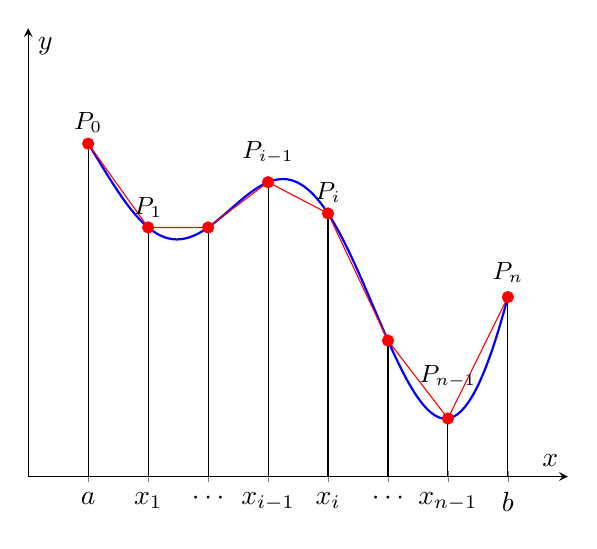
\begin{tikzpicture}
		\begin{axis}[axis lines = center, xmin = 0, xmax = 9, xlabel = $x$,
		xtick = {1, 2, 3, 4, 5, 6, 7, 8}, 
		xticklabels = {$a$, $x_1$,$\cdots$,$x_{i-1}$,$x_i$,$\cdots$,$x_{n-1}$,$b$},
		ymin = 0, 
            ymax = 9, 
            ylabel = $y$, ytick=\empty]
		\addplot[blue, thick, samples = 100, domain = 1:8]
            {(x-3)*(sin(57.296*x - 114.59))+5};
            \foreach \i in {1, 2, 3, 4, 5, 6, 7, 8}{
                \addplot[red, mark=*]coordinates{({\i},{(\i-3)*(sin(57.296*\i - 114.59))+5})};
                \addplot[black, thin]coordinates{({\i}, {0}) ({\i},{(\i-3)*(sin(57.296*\i - 114.59))+5})};
            }
            \foreach \i in {1, 2, 3, 4, 5, 6, 7}{
                \addplot[red, thin]coordinates{({\i},{(\i-3)*(sin(57.296*\i - 114.59))+5}) ({\i + 1}, {((\i+1)-3)*(sin(57.296*(\i+1) - 114.59))+5})};
            }
            \node[font = \small] at (1, 7.1) {$P_0$};
            \node[font = \small] at (2, 5.4) {$P_1$};
            \node[font = \small] at (4, 6.5) {$P_{i-1}$};
            \node[font = \small] at (5, 5.7) {$P_i$};
            \node[font = \small] at (7, 2) {$P_{n-1}$};
            \node[font = \small] at (8, 4.1) {$P_n$};
		\end{axis}
	\end{tikzpicture}
    \caption{Polygon approximation of $f(x)$}
    \label{fig:polygon}
\end{figure}

\begin{figure}[htbp]
\centering
	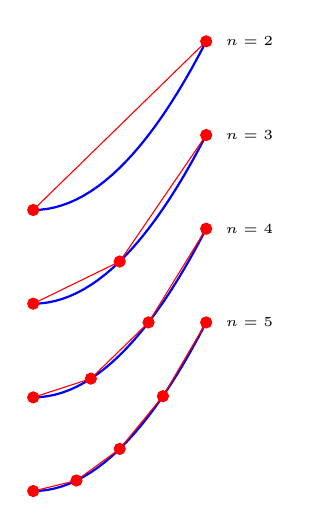
\begin{tikzpicture}
		\begin{axis}[axis lines = none, width=0.5*\axisdefaultwidth, height=\axisdefaultwidth, clip = false]
                \addplot[blue, thick, domain = 0:3]{x^2};
                \addplot[red, mark=*] coordinates {(0, 0) (0.75, 0.5625) (1.5, 2.25) (2.25, 5.0625) (3, 9)};
                \node[font = \tiny] at (3.75,9) {$n=5$};
                \addplot[blue, thick, domain = 0:3]{x^2+5};
                \addplot[red, mark=*] coordinates {(0, 5) (1, 6) (2, 9) (3, 14)};
                \node[font = \tiny] at (3.75,14) {$n=4$};
                \addplot[blue, thick, domain = 0:3]{x^2+10};
                \addplot[red, mark=*] coordinates {(0, 10) (1.5, 12.25) (3, 19)};
                \node[font = \tiny] at (3.75,19) {$n=3$};
                \addplot[blue, thick, domain = 0:3]{x^2+15};
                \addplot[red, mark=*] coordinates {(0, 15) (3, 24)};
                \node[font = \tiny] at (3.75,24) {$n=2$};
            \end{axis}
	\end{tikzpicture}
    \caption{As the number of points increases, the total length of the lines segments approaches the true length of the curve}
    \label{fig:points}
\end{figure}

The more points we choose, the closer the lines lay to the actual 
curve (see figure \ref{fig:points}), and the closer our estimate is 
to the true length. So, to find the true length, we will want to take 
$n$ to $\infty$. Therefore, the actual curve length is the limit as 
$n \to \infty$ of that sum:
$$L = \lim_{n \to \infty}\sum_{i=1}^n |P_{i-1}P_i|$$

The length of each segment can be found using the Pythgorean theorem. 
Recall that the distance between two points on the $xy$-plane is 
$\sqrt{(x_2 - x_1)^2 + (y_2 - y_1)^2}$. (For a reminder of why this 
is, see figure \ref{fig:distance}.) The coordinates of $P_{i-1}$ are 
$(x_{i-1}, f(x_{i-1}))$ and the coordinates of $P_i$ are $(x_i, 
f(x_i))$. Substituting this into the above sum, we see that the total 
length of the segments is 
$$\sum_{i=1}^n \sqrt{(x_i - x_{i-1})^2 + (f(x_i) - f(x_{i-1}))^2}$$

\begin{figure}[htbp]
\centering
	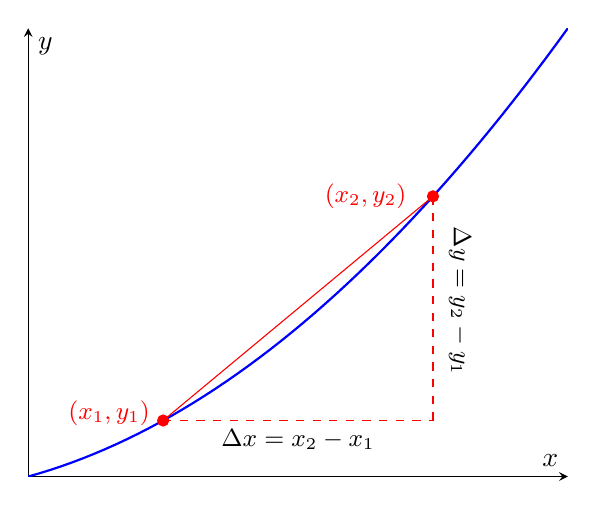
\begin{tikzpicture}
		\begin{axis}[axis lines = center, xlabel=$x$, ylabel=$y$, 
		xtick=\empty, ytick=\empty]
                \addplot[blue, thick, samples=50, domain = 0.5:2.5]
                {x^2};
                \addplot[red, thin, mark=*]coordinates{(1, 1) (2, 4)};
                \draw[red, thin, dashed](1,1) -- (2, 1);
                \draw[red, thin, dashed](2,1) -- (2, 4);
                \node[font=\small] at (1.5,0.75) 
                {$\Delta x = x_2 - x_1$};
                \node[font = \small, rotate = -90] at (2.1, 2.6) 
                {$\Delta y = y_2 - y_1$};
                \node[red, font = \small] at (0.8,1.1) {$(x_1, y_1)$};
                \node[red, font = \small] at (1.75, 4) {$(x_2, y_2)$};
            \end{axis}
	\end{tikzpicture}
    \caption{The distance between two points on the $xy$-plane}
    \label{fig:distance}
\end{figure}

Recall the Mean Value Theorem, which states that there is some 
$x_i^{\text{*}}$ such that $f(x_i) - f(x_{i-1}) = f'(x_i^{\text{*}})
(x_i - x_{i-1})$. Substituting this into the above sum, we get: 
$$\sum_{i=1}^n \sqrt{(x_i - x_{i-1})^2 + (f'(x_i^{\text{*}})(x_i - x_{i-1}))^2}$$ 
Recall from the chapter on Riemann sums and the integral that we 
defined $\Delta x = x_i - x_{i-1}$ and we can further re-write the 
sum as $$\sum_{i=1}^n \sqrt{(\Delta x)^2 + [f'(x_i^{\text{*}}) \Delta x]^2} 
= \sum_{i=1}^n \sqrt{1+[f'(x_i^{\text{*}})]^2}\sqrt{(\Delta x)^2} = 
\sum_{i=1}^n \sqrt{1+[f'(x_i^{\text{*}})]^2}\Delta x$$

Putting this all together, we see that that actual length of the 
curve is defined as $$L = \lim_{n \to \infty}\sum_{i=1}^n \sqrt{1+
[f'(x_i^{\text{*}})]^2}\Delta x$$

This is the definition of the integral of $\sqrt{1+[f'(x)]^2}$ and 
therefore the length of some function $f(x)$ on the interval $a < x <b$ 
is $\int_a^b \sqrt{1 + [f'(x)]^2}\,dx$. In another notation, this is 
equivalent to $\int_a^b \sqrt{1 + (\frac{dy}{dx})^2}\,dx$. 

\section{Arc Length of Vector-valued Functions}
Suppose you have a vector-valued function, $f(t) = [x(t), y(t)]$. A 
common example might be an artillery shell shot at an angle. For a 
shell shot with an initial velocity $v_o$ at angle $\theta$ from the 
ground, its position can be described with the vector-valued function 
$f(t) = [v_o\cos{\theta}(t), v_o\sin{\theta}(t) - 4.9t^2]$. (A 
concrete example where $v_o = 12 \frac{m}{s}$ and $\theta = 30^o$ is 
shown in figure \ref{fig:shell}.)

\begin{figure}[htbp]
\centering
	\begin{tikzpicture}
		\begin{axis}[axis lines = center, xlabel = $x$, ylabel = $y$]
                \addplot[blue, thick, domain = 0:1.22, samples = 100]
                ({12*cos(30)*x}, {12*sin(30)*x - 4.9*x^2});
            \end{axis}
	\end{tikzpicture}
    \caption{The path of an artillery shell with shot with initial 
    velocity $v_o$ at angle $\theta$}
    \label{fig:shell}
\end{figure}  

How can we find the length of the flight path of the artillery shell? 
We can re-interpret the length integral for a vector-valued function, 
$f(t) = [x(t), y(t)]$.  
$$L = \int_a^b \sqrt{1+(\frac{dy}{dx})^2}\,dx = 
\int_a^b \sqrt{1 + \frac{(dy/dt)^2}{(dx/dt)^2}}\frac{dx}{dt}\,dt$$\\
Moving the $\frac{dx}{dt}$ under the square root, we see that
$$L = \int_a^b \sqrt{(\frac{dx}{dt})^2 + (\frac{dy}{dt})^2}\,dt$$\\
Which is equivalent to 
$$L = \int_a^b \sqrt{(x'(t))^2 + (y'(t))^2}\,dx$$

\section{Applications in Physics}
When we take the integral of a velocity function, we get the 
\textit{displacement}. For example, if you drove to school and home 
again, your displacement would be zero. However, the \textit{distance} 
you traveled is not zero! We can use the arc length formula to find 
the total distance traveled. (Remember, that if $x(t)$ is the object's 
position, then its velocity is given by $x'(t)$.)

Suppose a block is attached to a spring on a frictionless horizontal 
surface. You pull on the block, initiating harmonic motion described 
by $v(t) = (-0.16)\sin{9t}$, where $v$ is in $\frac{m}{s}$ and $t$ is 
in $sec$. (Note: we are working in radians, not degrees.) What is the 
block's displacement from $t = 0$ to $t = 3$? What is the total 
distance the block moves from $t = 0$ to $t = 3$? 

To find the displacement, we integrate the velocity function over the 
specified interval:
$$\int_0^3 (-0.16)\sin{9t}\,dt = \frac{-0.16}{9}(-\cos{9t})|_0^3$$
$$=\frac{0.16}{9}[\cos{27} - \cos{0}] = \frac{(0.16)(-0.29 - 1)}{9} 
= -0.0229 m$$

The position function and displacement are shown in figure 
\ref{fig:block}. To find the total distance traveled, we need to find 
the length of the curve. Before we do so, take a minute to mentally 
predict: will the distance be more or less than the displacement?

\begin{figure}[htbp]
\centering
	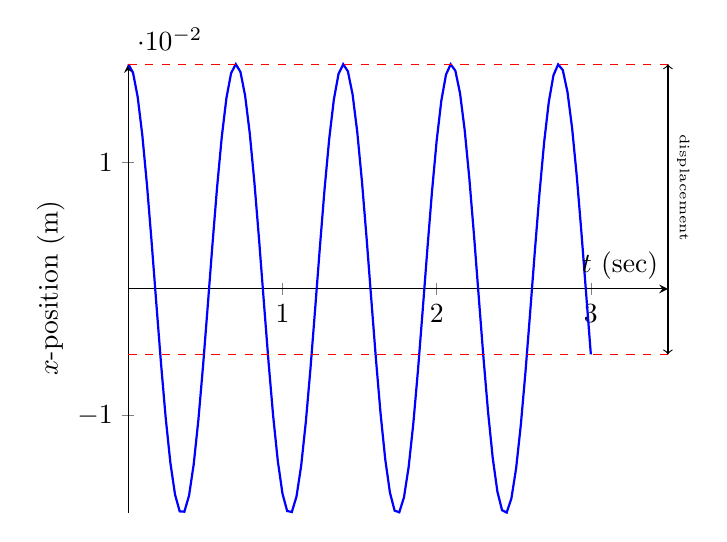
\begin{tikzpicture}
		\begin{axis}[axis lines = center, xlabel = $t$ (sec), 
		y label style={at={(axis description cs:-0.1,.5)},rotate=90,
		anchor=south}, ylabel = $x$-position (m), xmax = 3.5, clip = false, 
		xtick = {1, 2, 3}]
                \addplot[blue, thick, domain = 0:3, samples = 100]
                {0.01778*cos(9*deg(x))};
                \addplot[red, dashed] 
                coordinates {(0,0.01778) (3.5, 0.01778)};
                \addplot[red, dashed] 
                coordinates {(0, -0.00519) (3.5, -0.00519)};
                \draw[<->, black] (3.5, 0.01778) -- (3.5, -0.00519);
                \node[font=\tiny, rotate=-90] at (3.6, 0.008) 
                {displacement};
            \end{axis}
	\end{tikzpicture}
    \caption{The position of the block with displacement shown. The 
    distance traveled is the total length of the curve}
    \label{fig:block}
\end{figure}

Recalling that the distance traveled by an object is 
$\int_a^b \sqrt{1+[x'(t)]^2}\,dt = \int_a^b \sqrt{1 + [v(t)]^2}\,dt$, 
we can write an integral to determine the total distance traveled by the block:
$$\int_0^3 \sqrt{1 + [-0.16\sin{9t}]^2}\,dt$$

Unfortunately, we do not know an antiderivative for this integral, and 
$u$-substitution won't help us. However, for definite integrals, 
calculators such as a TI-89 or Wolfram Alpha can easily use Riemann 
sums to determine the value of the integral to a high precision. Using 
such a tool, we find that the total distance traveled by the block is 
$\approx$ 3.019 meters. Did you predict that the distance would be 
greater than the displacement?

\section{Practice}

\begin{Exercise}[label=length1]
Write an integral that gives the length of the requested curve.
	\begin{enumerate}
	\item $y = \ln{x}$ from $x = 1$ to $x = 3$
	\item $y = \sin{x}$ from $x = 0$ to $x = \pi$
	\item $y = \frac{x^3}{3} + \frac{1}{4x}$ from $x = 1$ to $x = 4$
	\item $y = \ln{(\cos{x})}$ from $x = 0$ to $x = \frac{\pi}{3}$
	\end{enumerate}	 
\end{Exercise}

\begin{Answer}[ref=length1]
	\begin{enumerate}
	\item $L = \int_{1}^{3} \sqrt{1 + \frac{1}{x^2}}\,dx$
	\item $L = \int_{0}^{\pi} \sqrt{1 + \cos^2{x}}\,dx$
	\item $L = \int_{1}^{4} \sqrt{1 + (x^2-\frac{1}{4x^2})^2}\,dx$
	\item $L = \int_{0}^{\frac{\pi}{3}} \sqrt{1 + (\frac{1}{\cos{x}} 
	\times - \sin{x})^2}\,dx = \int_{0}^{\frac{\pi}{3}} \sqrt{1 + 
	\tan^2{x}}\,dx$
	\end{enumerate}
\end{Answer}

\begin{Exercise}[label=length2]
The arc length function for a curve $f(x)$, where $f$ is an increasing 
function, is given by $s(x) = \int_{0}^{x} \sqrt{3t + 5}\,dt$. If $f$ 
has $y$-intercept 2, find an equation for $f$. What point on $f$ is 
three units from the $y$-intercept? Give your answer to the thousandths 
place. 
\end{Exercise}

\begin{Answer}[ref=length2]
From looking at the structure of the given arc length integral, we can 
see that $f'(t) = \sqrt{3t + 4}$. Taking the antiderivative, we find 
that $f(x) = \frac{2}{9}(3x + 4)^{3 / 2} + C$. Substituting $f(0) = 2$
, we can solve for $C$. $$2 = \frac{2}{9}(3(0) + 4)^{3 / 2} + C$$ 
$$2 = \frac{2}{9}(4)^{3 / 2} + C$$ 
$$2 = \frac{2}{9}(2)^3 + C$$ 
$$2 = \frac{16}{9} + C$$ 
$$\frac{18}{9} = \frac{16 + 9C}{9}$$ 
$$18 = 16 + 9C$$ 
$$2 = 9C$$ 
$$C = \frac{2}{9}$$\\ 
Therefore, $f(x) = \frac{2}{3}(3x + 4)^{3 / 2} + \frac{2}{9}$. To find 
the coordinate point where $s(x) = 3$, we first note that the 
antiderivative of $\sqrt{3t + 5}$ is $\frac{2}{9}(3t + 5)^{3 / 2} + C$. 
Therefore, $s(x) = \frac{2}{9}(3x + 5)^{3 / 2} - \frac{2}{9}(5)^{3 / 2}$. 
Setting $s(x) = 3$ and solving for $x$, we find that $x = 1.159$
\end{Answer}

\begin{Exercise}[label=length3]
	[This problem was originally presented as a no-calculator, 
	multiple-choice question on the 2012 AP Calculus BC exam.] Write an 
	integral that gives the length of the curve $ y = \ln{x}$ from 
	$x = 1$ to $x = 2$. 
\end{Exercise}

\begin{Answer}[ref=length3]
Recall that arc length is given by $\int_a^b \sqrt{1 + [f'(x)]^2}\,dx$. 
Since $f(x) = \ln{x}$, then $f'(x) = \frac{1}{x}$. Taking $a = 1$, 
$b = 2$, and $f'(x) = \frac{1}{x}$, the integral that gives the length 
of the curve $y = \ln{x}$ on the specified interval is $\int_1^2 
\sqrt{1+\frac{1}{x^2}}\,dx$. 
\end{Answer}

\begin{Exercise}[label = length4]
	An out of control rocket ship is spiraling out of control through 
	space. Its velocity can be described with the vector-valued function 
	$v(t) = [-1412\sin{t}, 1412\cos{t}, t]$ where $v$ is in $\frac{m}{s}$ 
	and $t$ is in $sec$. How far does the ship travel in the first 60 
	seconds? In the second 60 seconds? [Hint: in three dimensions, the 
	length of a vector-valued function is $\int_a^b 
	\sqrt{(\frac{dx}{dt})^2 + (\frac{dy}{dt})^2 + (\frac{dz}{dt})^2}\,dt$]
\end{Exercise}

\begin{Answer}[ref= length4]
	Since we are told the vector-valued velocity of the ship, we know 
	that $\frac{dx}{dt} = -1412\sin{t}$, $\frac{dy}{dt} = 1412\cos{t}$, 
	and $\frac{dz}{dt} = t$. The distance traveled in the first 60 
	seconds is given by $\int_0^{60} \sqrt{(-1412\sin{t})^2 + 
	(1412\cos{t})^2 + t^2}\,dt$. Using a calculator, the integral 
	evaluates to $84745$ meters. The distance traveled in the second 60 
	seconds is given by \\$\int_{60}^{120} \sqrt{(-1412\sin{t})^2 + 
	(1412\cos{t})^2 + t^2}\,dt$. Using a calculator, this integral 
	evaluates to $84898$ meters.
\end{Answer}






